\documentclass[english]{exercisesheet}

\usepackage{bm}
\usepackage{mymath}
\usepackage{graphicx}

\author{Lorenzo Minecci, Daniel Strenger}
\immatriculationnumber{11939539, 01531211}
\semester{SS 2020}
\subject{Machine Learning}
\sheetnumber{2}

\begin{document}
 \makedocumentheader
 
 \begin{nexercise}{Logistic Regression}
\end{nexercise}

\begin{solution}
 1. We have $p(t=1|\bm{\tilde{x}})=\sigma(\bm{\tilde{w}}^t\bm{\tilde{x}})=\sigma(1\cdot\bm{w}^t\bm{\tilde{x}})$ and

 \begin{align*}
 p(t=-1|\bm{\tilde{x}})=1-\sigma(\bm{\tilde{w}}^t\bm{\tilde{x}})=1-\frac{1}{1+e^{-\bm{\tilde{w}}^t\bm{\tilde{x}}}}=\frac{1+e^{-\bm{\tilde{w}}^t\bm{\tilde{x}}}}{1+e^{-\bm{\tilde{w}}^t\bm{\tilde{x}}}}-\frac{1}{1+e^{-\bm{\tilde{w}}^t\bm{\tilde{x}}}}\\=\frac{e^{-\bm{\tilde{w}}^t\bm{\tilde{x}}}}{1+e^{-\bm{\tilde{w}}^t\bm{\tilde{x}}}}=\frac{1}{e^{\bm{\tilde{w}}^t\bm{\tilde{x}}}+1}=\sigma(-\bm{\tilde{w}}^t\bm{\tilde{x}})
\end{align*}\\
\par 2.
\begin{align*}
 -\log (p(\bm{\tilde{w}}|\bm{t},\bm{x}))=-\log(p(\bm{w}))-\sum_{n=1}^N \log(\sigma(t_n\bm{\tilde{w}^t\tilde{x}_n}))=\\-\log(p(\bm{w}))-\sum_{n=1}^N \log(\frac{1}{1+e^{-t_n\bm{\tilde{w}^t\tilde{x}_n}}})\\
 =-\log(p(\bm{w}))+\sum_{n=1}^N \log(1+e^{-t_n\bm{\tilde{w}^t\tilde{x}_n}})=\\-\log\left(\frac{1}{(2\pi S^{2})^{N/2}}\exp\left(-\frac{1}{2S^{2}}\sum_{n=1}^N w_n^2\right)\right)+\sum_{n=1}^N \log(1+e^{-t_n\bm{\tilde{w}^t\tilde{x}_n}})\\
 =-\log\left(\frac{1}{(2\pi S^{2})^{N/2}}\right)+\frac{1}{2S^{2}}\sum_{n=1}^N w_n^2+\sum_{n=1}^N \log(1+e^{-t_n\bm{\tilde{w}^t\tilde{x}_n}})
\end{align*}\\
\par 3.
\begin{align*}
 \frac{\partial}{\partial b}E(\bm{\tilde{w}})=\sum_{n=1}^N\frac{\partial}{\partial b} \log(1+e^{-t_n\bm{\tilde{w}^t\tilde{x}_n}})=\sum_{n=1}^N\frac{-t_ne^{-t_n\bm{\tilde{w}^t\tilde{x}_n}}}{1+e^{-t_n\bm{\tilde{w}^t\tilde{x}_n}}},\\
 \frac{\partial}{\partial w_i}E(\bm{\tilde{w}})=\frac{1}{2S^{2}}\sum_{n=1}^N  \frac{\partial}{\partial w_i} w_n^2+\sum_{n=1}^N\frac{\partial}{\partial w_i} \log(1+e^{-t_n\bm{\tilde{w}^t\tilde{x}_n}})\\
 =\frac{w_i}{S^{2}}+\sum_{n=1}^N\frac{-t_n\tilde{x}_n^ie^{-t_n\bm{\tilde{w}^t\tilde{x}_n}}}{1+e^{-t_n\bm{\tilde{w}^t\tilde{x}_n}}}
\end{align*}
\\
\par 5. b)
\begin{figure}[h]
\centering
 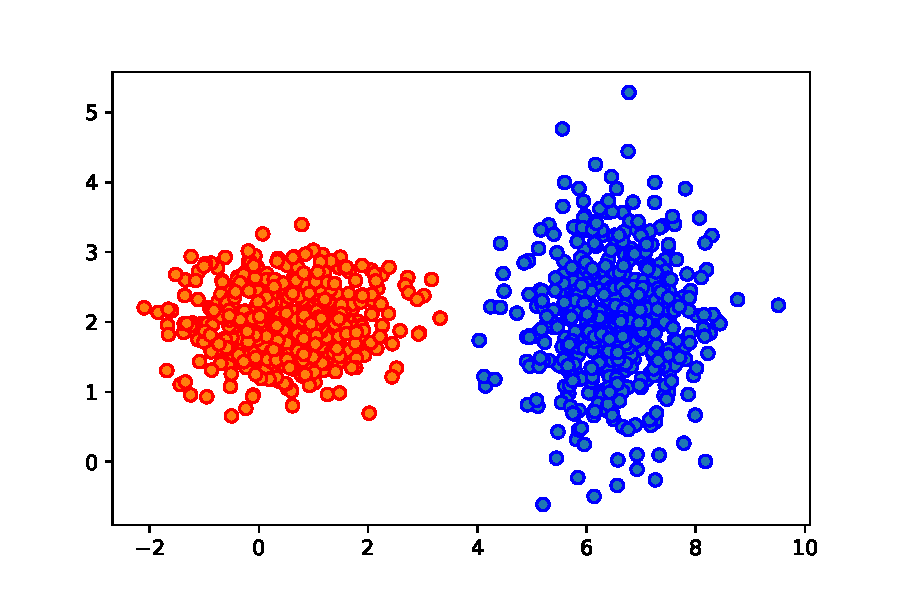
\includegraphics[width=0.7\textwidth]{points.pdf}
 \caption{The generated points}
\end{figure}

\par e,f) The decision boundary is the curve
\begin{align*}
 p(t=1|\bm{x})=0.5 \Leftrightarrow \frac{1}{1+e^{\bm{\tilde{w}^t\tilde{x}}}}=0.5\Leftrightarrow 1+e^{\bm{\tilde{w}^t\tilde{x}}}=2\Leftrightarrow \bm{\tilde{w}^t\tilde{x}}=\log(1)=0,
\end{align*}
so it is the line
\begin{equation*}
 y=-\frac{w_1}{w_2}x-\frac{b}{w_2}.
\end{equation*}

\begin{figure}
 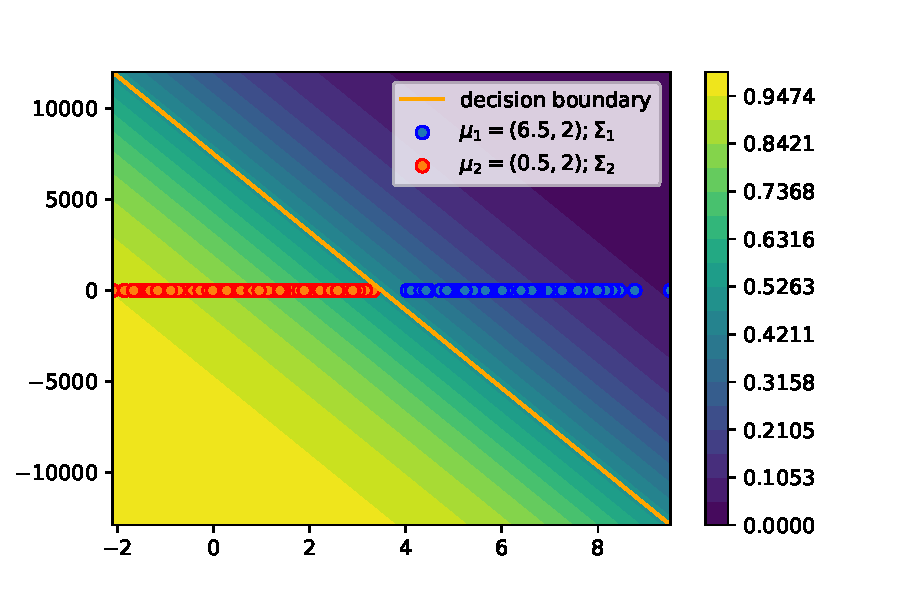
\includegraphics[width=0.5\textwidth]{simulated-1.pdf}
 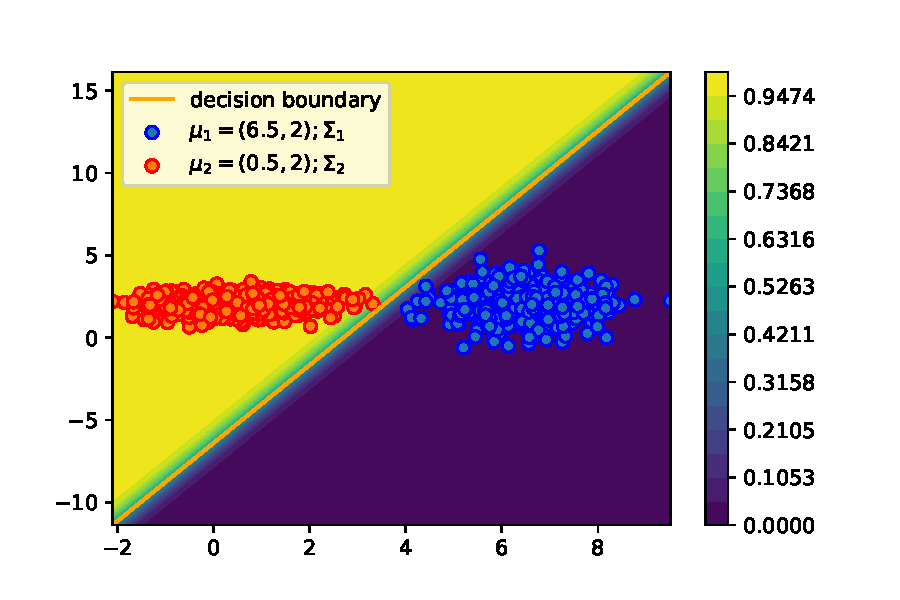
\includegraphics[width=0.5\textwidth]{simulated-8.pdf}
 \caption{decision boundary and probabilities for $S^2=10^{-3},10^4$}
\end{figure}
In this case the computed decision boundary really seperates the red and blue training points (for both values of $S^2$), although in some cases the points may not be linearly separable in two dimensions, which also happened in some tests. The probability around the decision boundary is about 0.5, which is clear, because the boundary was chosen for this reason. If a high variance for $\bm{w}$ is assumed, the probability decreases rather slowly when moving away from the decision boundary. For higher $S^2$ the probability decreases much faster and the predictions can be made with more certainty.\\
\par 6. The accuracy for variing $S^2$ is
\begin{table}[h]
\begin{tabular}{lll}
 $S^2$&training  &validation\\ \hline
 $10^{-4}$& 0.6088 & 0.6029 \\
 $10^{-3}$& 0.8435 & 0.8377 \\
 $10^{-2}$& 0.9003 & 0.8826 \\
 $10^{-1}$& 0.9193 & 0.9123 \\
 1& 0.9165 & 0.9152 \\
 $10^{1}$& 0.9169 & 0.9109 \\
 $10^{2}$& 0.9165 & 0.9145 \\
 $10^{3}$& 0.9143 & 0.9101 \\
 $10^{4}$& 0.9165 & 0.9138
\end{tabular}
\end{table}\\
It fits the previous observation that for higher $S^2$ the predictions can be made with more certainty, but this effect seems to be limited by $S^2 \approx 0.1$, after that no real improvement is achieved.
\end{solution}

 
\end{document}
